\chapter{Lab 1 - Setting Up the Development Environment}

In this lab, we'll set up the basic development environment for the rest of our labs. Firstly
I'll introduce you to the tools and we'll install them, then we'll compile MOS, run it in QEMU
for the first time, and then attach GDB to it.

Finally, and hopefully, you can get your favorite IDE set up to work with MOS.

\section{Introduction to the Tools}

MOS is an operating system, thus, preparing for a development environment is already not
an easy task (bruh). Several efforts have been made to make the process easier.

We are currently targeting the 32-bit \texttt{x86} architecture, the tools in table \ref{tab:tools}
are the ones we'll be using.

\begin{table}[h!]
    \centering
    \begin{tabular}{|l|c|c|}
        \hline \textbf{Tool}               & \textbf{Description}     & \textbf{Installation}            \\
        \hline \texttt{CMake}              & \ref{sec:cmake}          & \ref{sec:cmake-install}          \\
        \hline \texttt{i686-elf} toolchain & \ref{sec:cross-compiler} & \ref{sec:cross-compiler-install} \\
        \hline \texttt{NASM}               & \ref{sec:nasm}           & \ref{sec:nasm-install}           \\
        \hline \texttt{cpio}               & \ref{sec:cpio}           & \ref{sec:cpio-install}           \\
        \hline \texttt{qemu-system-i386}   & \ref{sec:qemu}           & \ref{sec:qemu-install}           \\
        \hline
    \end{tabular}
    \caption{Tools used in this lab}
    \label{tab:tools}
\end{table}

\subsection{CMake} \label{sec:cmake}

\begin{quote}
    CMake is an open-source, cross-platform family of tools designed to build, test and package
    software\footnote{https://cmake.org/}
\end{quote}

MOS uses CMake as the build system generator, it supports many build systems like `Make', `Ninja',
`Visual Studio' and `Xcode'.

\begin{note}
    \item It's the actual build system (e.g. `Make') that starts the compiler, linker, etc.,
    CMake is only to \textbf{generate} the configuration files for such build system.
\end{note}

We'll use `Make' as the build system for MOS in this tutorial, but
\textbf{you can use `Ninja' if you want}.

\subsection{NASM} \label{sec:nasm}

NASM is an assembler for x86 architecture. There are several files under `arch/x86`
that are written in NASM. It has a cleaner syntax than the GNU assembler (i.e. \texttt{as}).

\subsection{cpio} \label{sec:cpio}

Cpio is the format of an archive, and also the tool to create such archives. MOS uses cpio as
the initial root filesystem.

\subsection{qemu-system-i386} \label{sec:qemu}

QEMU is an open-source emulator, it also provides a gdb stub for debugging. It can be
installed via your Linux's package manager.

(e.g. \texttt{apt install qemu-system-i386} or \texttt{pacman -S qemu-system-x86}, \dots).

See its \href{https://www.qemu.org/download}{download page} for more details.

\subsection{i686-elf Toolchain} \label{sec:cross-compiler}

As its name suggests, this is a cross toolchain for `i686-elf' target. `i686' means the 32-bit
x86 architecture, and `elf' is the executable format. They together form the `target-triple' of
the toolchain.

\begin{tip}
    \item Most 64-bit Linux OSes have `target triple' of \texttt{x86\_64-pc-linux-gnu}, or
    \texttt{x86\_64-linux-gnu}.
    \item Read more about `target triple' at \url{https://wiki.osdev.org/Target_Triplet}.
\end{tip}

Unlike other applications (e.g. \texttt{bash} or \texttt{vim}) that they run on an existing
operating system and a standard C library (say, \texttt{glibc} or \texttt{musl}). MOS itself is
the operating system, thus there's not an existing OS for it to run on, neither a standard libc
(i.e. no \texttt{printf}, no \texttt{malloc} etc.) for it to use, considering you're directly
interacting with the CPU and the hardware.

This is called `bare-metal' environment, or `freestanding' environment, a `bare-metal' compiler
toolchain is exactly for this situation.

\begin{warning}
    \item One should never use a hosted compiler (e.g. the \texttt{gcc} installed on the lab machine)
    to cross-compile for a bare-metal environment when they are targeting a different architecture,
    (\texttt{x86} and \texttt{x86\_64} are different), it \textit{\textbf{may sometimes}} work, but
    you may encouter some weird bugs.

    \item See \url{https://wiki.osdev.org/Why_do_I_need_a_Cross_Compiler%3F}.
\end{warning}

\section{Installating the Tools}

\subsection{CMake} \label{sec:cmake-install}

CMake should come with your Linux distribution's package manager, MOS requires at least version
3.20, but any newer version is recommended.

\subsection{NASM} \label{sec:nasm-install}

NASM can be installed via your Linux's package manager, the minimum version of NASM tested is
\texttt{2.15.03}. A pre-built binary from \href{https://www.nasm.us}{NASM's website} is also
available.

\subsection{cpio} \label{sec:cpio-install}

cpio can also be installed via your Linux's package manager, the minimum version of cpio
tested is \texttt{2.12}.

\subsection{qemu-system-i386} \label{sec:qemu-install}

Major Linux distributions provides a package for QEMU, thus it's recommended to install it via
your Linux's package manager.

\subsection{i686-elf Toolchain} \label{sec:cross-compiler-install}

Installing the cross-compiler toolchain is probably the most difficult part of this lab,
but it's once and for all, you don't have to do it again (unless you want to upgrade the
toolchain).

There are majorly two ways to get this toolchain, either by building it from source or by
downloading a pre-built binary.

\subsubsection{Downloading a pre-built binary}

If you don't want to build the toolchain from source, you can download a pre-built
binary from
\href{https://github.com/moodyhunter/i686-elf-prebuilt/releases}{moodyhunter/i686-elf-prebuilt}
(choose the i686 one).

\begin{warning}
    \item Using pre-built binary saves time, but please consider doing so \textbf{only} if you
    trust the author.
    \item The pre-built binary is built on Ubuntu, it \textbf{may not} work on other Linux
    distributions, so the author \textbf{strongly} recommends you to build the toolchain from
    source, see next section.
\end{warning}

\subsubsection{Building From Source}

The source code of binutils and gcc can be found at
\href{https://www.gnu.org/software/binutils}{GNU Binutils's Website} and
\href{https://gcc.gnu.org}{GNU GCC's Website} respectively.

The script located at \texttt{docs/assets/i686-elf-toolchain.sh} downloads, compiles and
installs the toolchain into the directory specified by the \texttt{PREFIX} variable.

It is not suggested to install the toolchain to a system directory (e.g. \texttt{/usr}),
because it may cause conflicts with the system's package manager.

\section{Building MOS}

\begin{note}
    \item \texttt{PATH} is an environment variable that specifies a set of directories, separated
    by \texttt{:}, to search for executable files in response to commands issued by a user.
    \item Before you continue reading, make sure \texttt{i686-elf-gcc}, \texttt{i686-elf-ld},
    \texttt{nasm}, \texttt{cpio} are in your \texttt{PATH}. You can use the command below to check:
    \begin{minted}{bash}
    $ echo $PATH
    \end{minted}
    and use the command below to add them to your \texttt{PATH}:
    \begin{minted}{bash}
    $ export PATH="/TO/TOOLCHAINS/bin:$PATH"
    \end{minted}
    and use the command below to check if they are in your \texttt{PATH}:
    \begin{minted}{bash}
    $ which i686-elf-gcc
    $ which i686-elf-ld
    $ which nasm
    $ which cpio
    \end{minted}
\end{note}

\subsection{Cloning the Repository}

The recommended way to get MOS is to clone the repository from GitHub:

\begin{verbatim}
    git clone https://github.com/moodyhunter/MOS
    cd MOS
\end{verbatim}

\subsection{Configuring MOS}

If you have a correct setup, then configuring step should be as simple as:

\begin{verbatim}
    $ mkdir build && cd build
    $ cmake ..
\end{verbatim}

The first line creates a build directory, we are not going to build MOS in the source directory
directly, because there will be many generated files, and it's not a good idea to pollute the
source directory.

The second line runs CMake to configure MOS, after running this command, you should see a
bunch of output, similar to \ref{fig:cmake-output}.

\begin{figure}[ht]
    \centering
    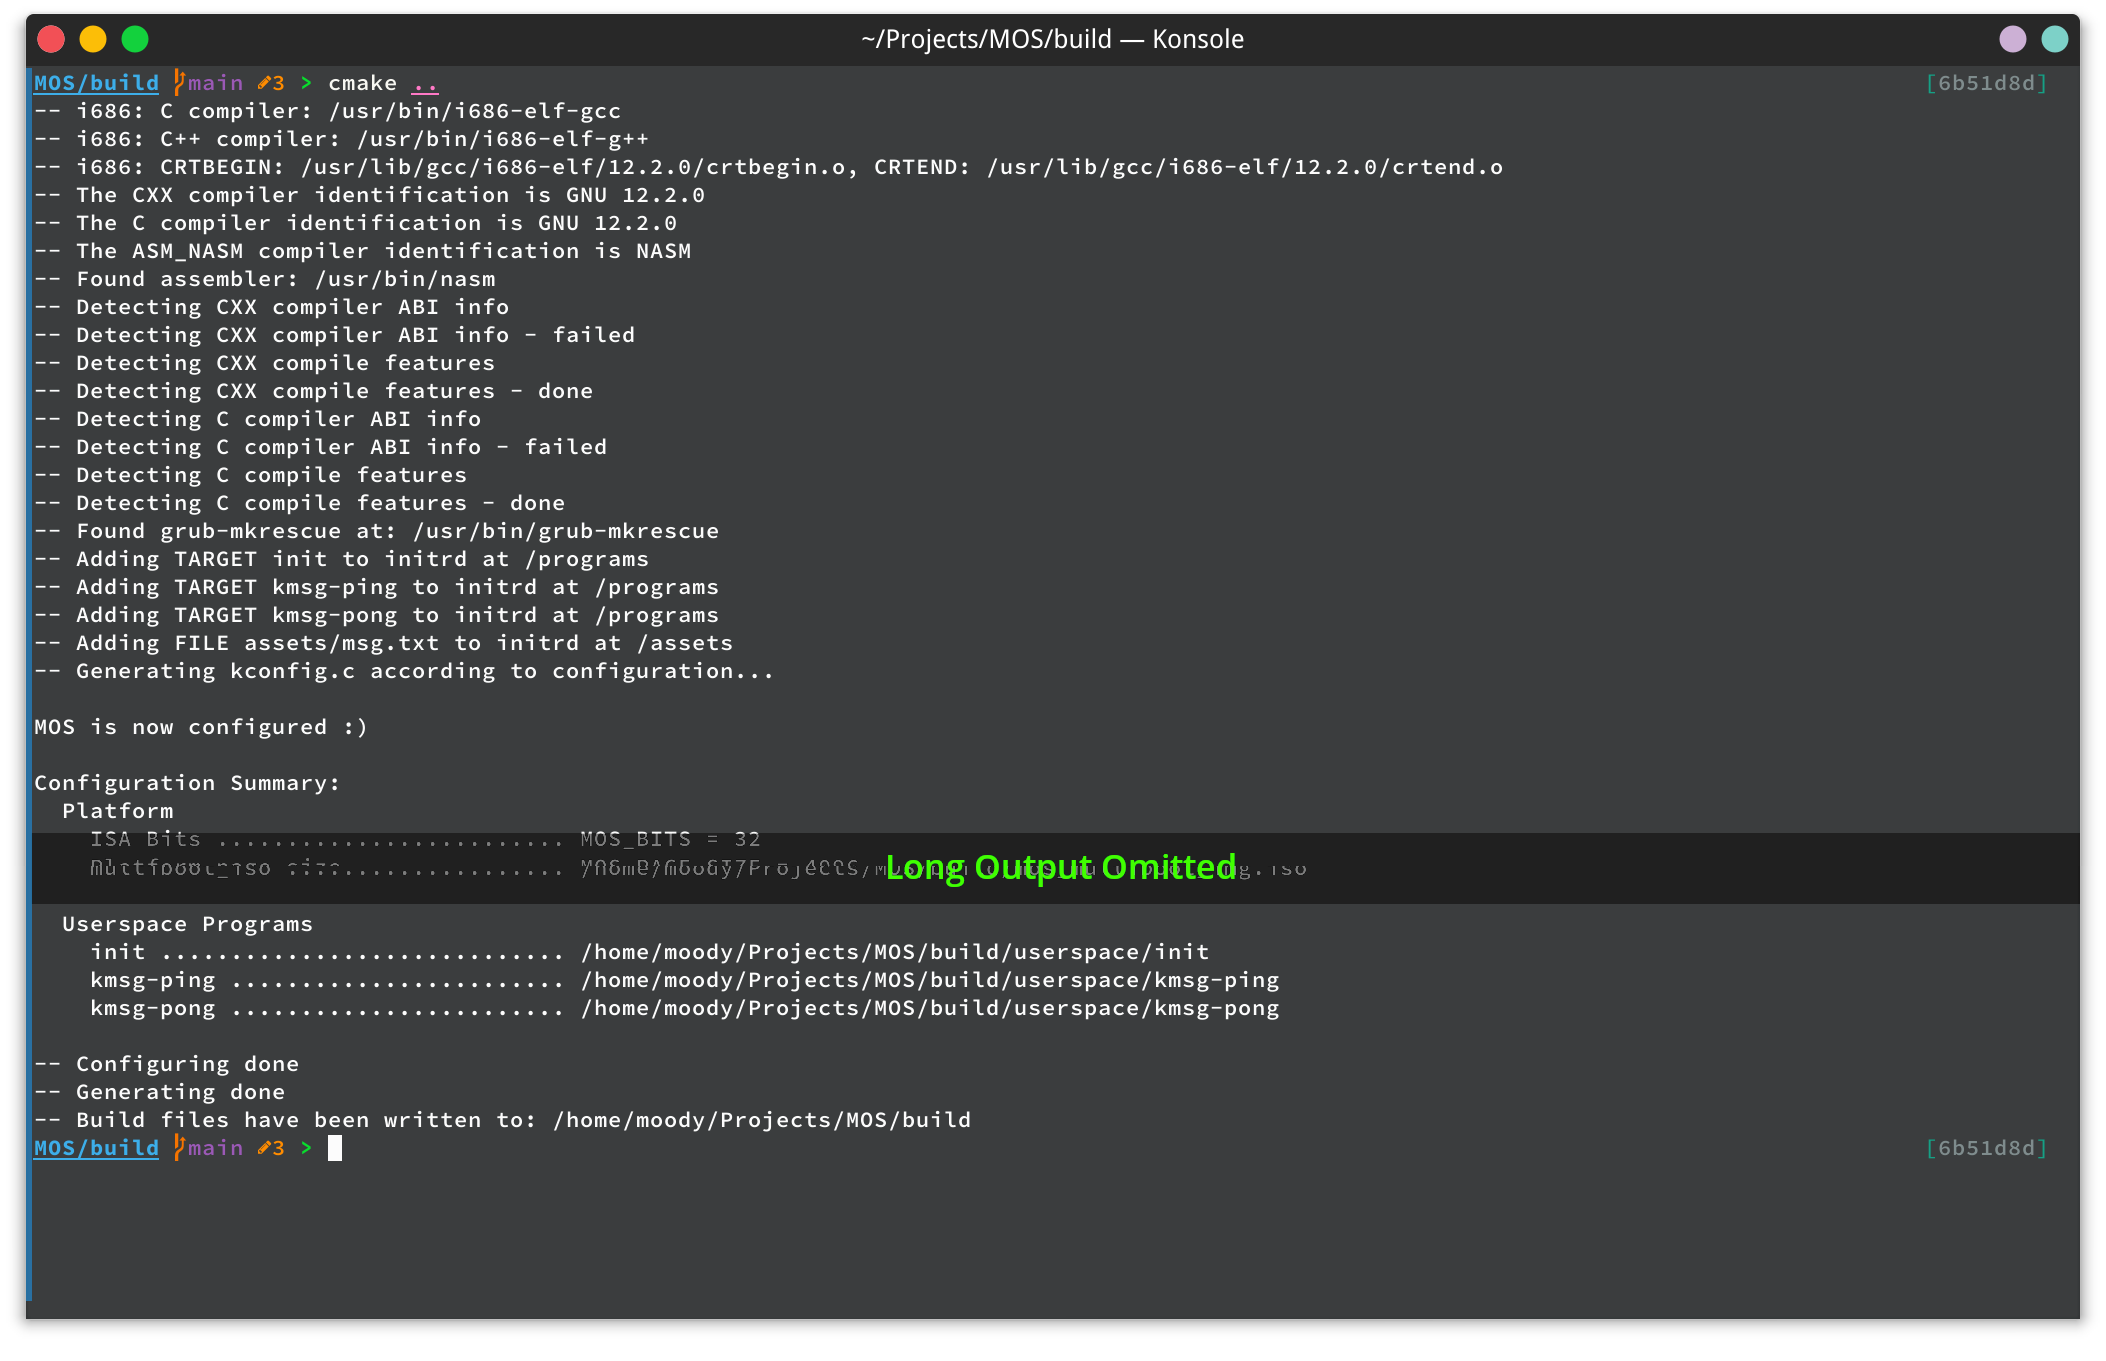
\includegraphics[width=\textwidth]{assets/c1.mos-cmake-configure.png}
    \caption{CMake Output}
    \label{fig:cmake-output}
\end{figure}

Don't worry if you see \texttt{C compiler ABI info} and \texttt{CXX compiler ABI info}
fails, it's because CMake doesn't know what to do with a cross compiler, this check is meaningless.

You may also see \texttt{grub-mkrescue} is not found, don't worry as well :), we are not going to use it.

If you don't see the \texttt{-- Configuring done} or \texttt{-- Generating done} line, then
something has been wrong, and you should scroll up and see what's wrong.

The \texttt{build} directory is where all the generated files are located, you can safely
delete it and re-run CMake to re-generate the files, in case you messed up something.

\subsection{Building MOS}

After configuring MOS, you can build MOS by running \texttt{make}.

This command will only build the core part of MOS, which is the kernel and the userspace library.
See the table below for an example list of targets.

\begin{tip}
    \item Think of a ``target'' as a deliverable, for example, building the \texttt{mos\_kernel} target
    will produce a kernel binary, building the \texttt{mos\_userspace\_programs} will ensure
    all the userspace programs are built.
\end{tip}

\begin{table}[ht]
    \centering
    \small
    \begin{tabular}{|l|l|l|}
        \hline
        \textbf{Target}      & \textbf{Description} & \textbf{Depends on}    \\ \hline
        \texttt{mos\_kernel} & Bare kernel          & \textit{None}          \\ \hline
        \texttt{mos\_initrd} & The initial ramdisk  & All userspace programs \\ \hline
        \texttt{multiboot}   & A bootable kernel    & \texttt{mos\_kernel}   \\ \hline
    \end{tabular} \\
    \begin{note}
        \item This is not a complete list.
        \item For a complete list of targets, you can look at the \texttt{summary.txt} in the \texttt{build} directory,
        and see the ``\texttt{Userspace Targets}'', ``\texttt{Utility Targets}'' and ``\texttt{Bootable Targets}'' section.
    \end{note}
    \caption{Targets}
    \label{tab:targets}
\end{table}

We are going to build the \texttt{multiboot} and \texttt{mos\_initrd} targets, these are the two
`utility' targets that 1) produce a bootable kernel and 2) create an initrd image.

An `initrd' is a compressed archive that contains our userspace programs, it literally means ``initial ramdisk'',
that is, the disk image that is loaded into the RAM when the kernel boots.

So the command will be \texttt{make multiboot mos\_initrd} (replace \texttt{make} with \texttt{ninja} if you are using Ninja).

You'll then see two files being generated in the \texttt{build} directory:

\begin{itemize}
    \item \texttt{mos\_multiboot.bin} is the kernel image, which is a multiboot-compliant kernel.
    \item \texttt{initrd.cpio} is the initrd image, which contains the userspace programs.
\end{itemize}

Several other files are also generated, for more information, read the MOS documentation, section \texttt{CMake Targets}.

\begin{exercise}
    \item Use the utility target \texttt{mos\_print\_summary} to print a summary of all the targets.
    \item Navigate to \texttt{initrd} under the build directory, and use \texttt{find .} to list all the files.
\end{exercise}

\section{Running MOS}

Once we have compiled MOS, we can run it in QEMU.

The command passed to QEMU will be flexible based on your needs, but the most basic command is:

\begin{verbatim}
    qemu-system-i386 -m 4G -kernel mos_multiboot.bin -initrd initrd.cpio -serial stdio
\end{verbatim}

You can pass more arguments to QEMU:

\begin{itemize}
    \item \texttt{-s} to enable the QEMU GDB stub, which allows you to debug MOS using GDB.
    \item \texttt{-S} to pause the CPU before starting up, which allows GDB to take control of
          the booting process.
    \item \texttt{-m} to specify the amount of RAM to be allocated to the VM (say \texttt{-m 512M}).
          the preferred amount of RAM is 4GB, less RAM may cause the kernel to fail.
    \item \texttt{-append} to pass arguments to the kernel, several arguments are:
          \begin{itemize}
              \item \texttt{quiet}: suppress (most-of) all non-warning kernel messages.
              \item \texttt{init=}: path to the init program, e.g. \texttt{init=/initrd/programs/mossh}.
          \end{itemize}
          For a complete list of supported arguments, see the MOS documentation section.
    \item \dots For more possible arguments, you may want to read QEMU's documentation.
\end{itemize}

\begin{tip}
    \item If you accidentally specified \texttt{-nographic} to QEMU and find that you can't terminate
    the QEMU process by pressing \texttt{Ctrl+C}. You can press \texttt{Ctrl+A} and then \texttt{x}
    instead to achieve the same effect. (Press \texttt{Ctrl+A} and then \texttt{h} to see a list of these
    shortcuts.)
\end{tip}

\begin{exercise}
    \item Run MOS with the command above.
    \item Run MOS with \texttt{-m 3G} and \texttt{-m 512M}, what's the difference?
\end{exercise}

\section{Debugging MOS}

After successfully building and running MOS, you may want to debug it (just in case your code crashes
the kernel).

\subsection{Required QEMU Arguments} \label{sec:qemu-args}

As mentioned above, we need to pass 2 more arguments \texttt{-s} and \texttt{-S} to QEMU so that it
1) enables the GDB stub, and 2) pauses the CPU before starting up (so that we have time to attach and
place breakpoints).

After adding these two arguments, when starting up QEMU, you will see a message like Figure \ref{fig:qemu-gdb-paused}.

\begin{figure}[h]
    \centering
    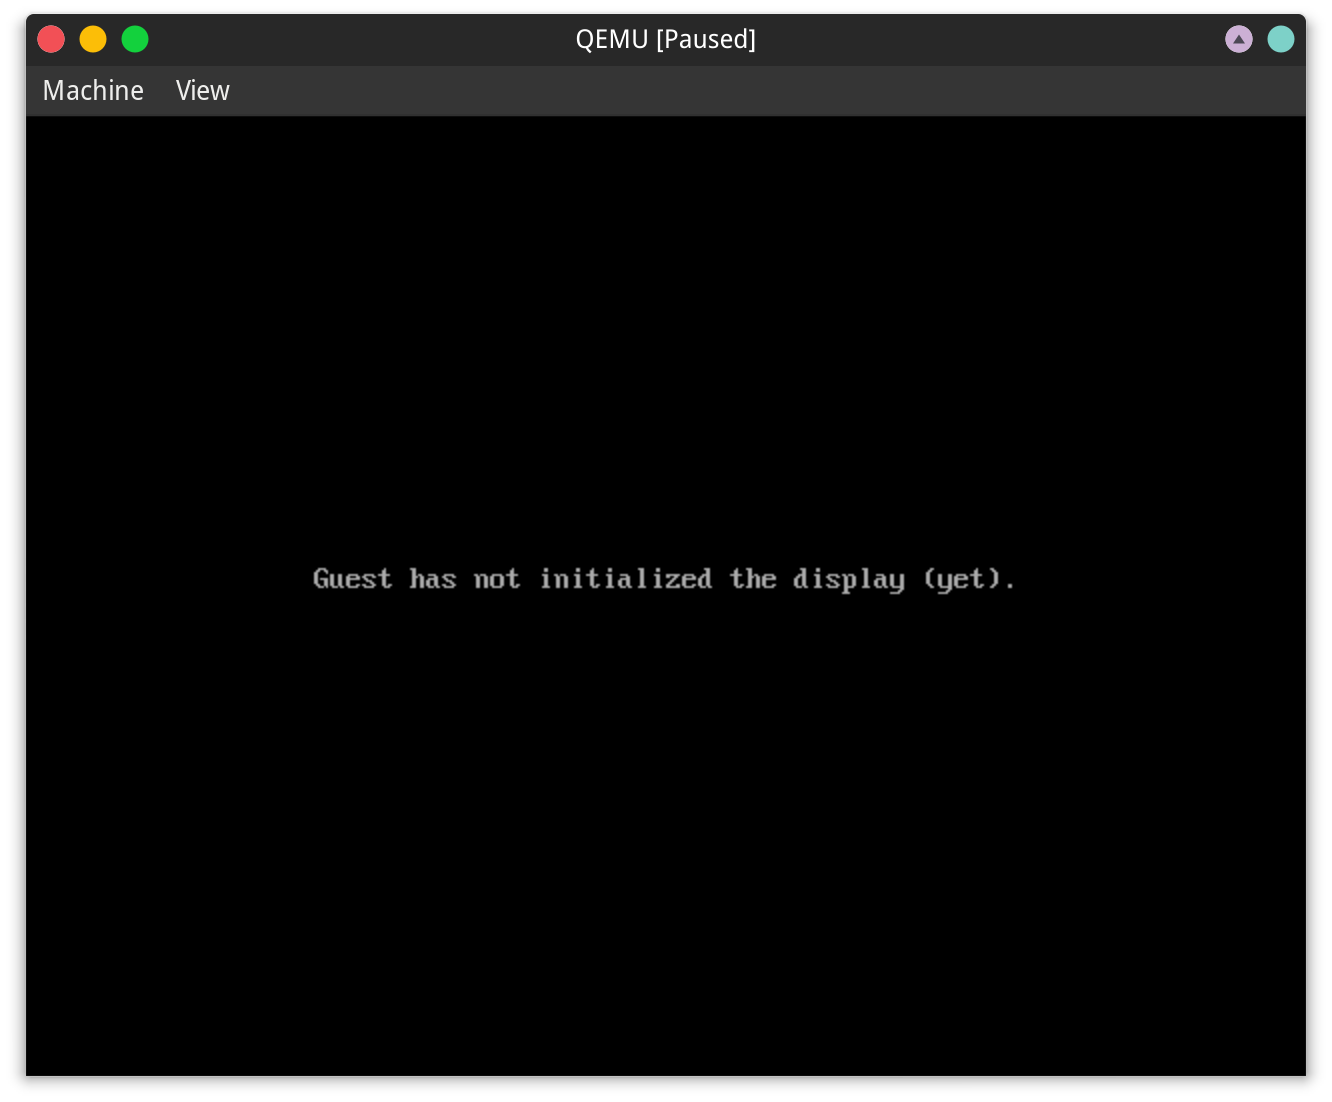
\includegraphics[width=\textwidth]{assets/c1.mos-qemu-gdb-paused.png}
    \caption{QEMU GDB in Paused State}
    \label{fig:qemu-gdb-paused}
\end{figure}

This means that QEMU is waiting for a GDB connection, and we can now continue to the next step.

\subsection{Configuring GDB} \label{sec:gdb-config}

Note that we are targeting the \texttt{i686-elf} architecture, so you should use \texttt{i686-elf-gdb}
instead of \texttt{gdb}.

To begin with, we need to tell GDB where the kernel file is, so that GDB can load debug information
from it.

You've probably already seen a \texttt{gdbinit} file in the \texttt{build} directory. This file
contains commands for GDB to recognize our userspace programs, we'll pass this file to GDB using
the \texttt{-x} argument.

So the overall command will be:

\begin{verbatim}
    i686-elf-gdb ./mos_multiboot.bin -x ./gdbinit
\end{verbatim}

\subsection{Attaching to QEMU} \label{sec:gdb-attach}

After GDB starts, you'll see it's `adding symbol table from file' thanks to our \texttt{gdbinit} file.
Now we need to attach GDB to QEMU, so that we can place breakpoints and debug the kernel.

QEMU (by default) listens on port 1234 for GDB connections, so we need to tell GDB to connect to it:

\begin{verbatim}
    (gdb) target remote localhost:1234
\end{verbatim}

GDB will then connect to QEMU, and you'll see a message like Figure \ref{fig:gdb-attached}.

\begin{figure}[ht]
    \centering
    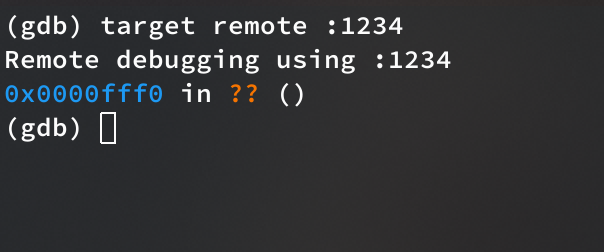
\includegraphics[width=\textwidth]{assets/c1.gdb-attached.png}
    \caption{GDB Attached to QEMU}
    \label{fig:gdb-attached}
\end{figure}

Try typing \texttt{break main} and then \texttt{continue} to see if it pauses at the \texttt{main}
function, you should see a message like Figure \ref{fig:gdb-paused}.

\begin{figure}[ht]
    \centering
    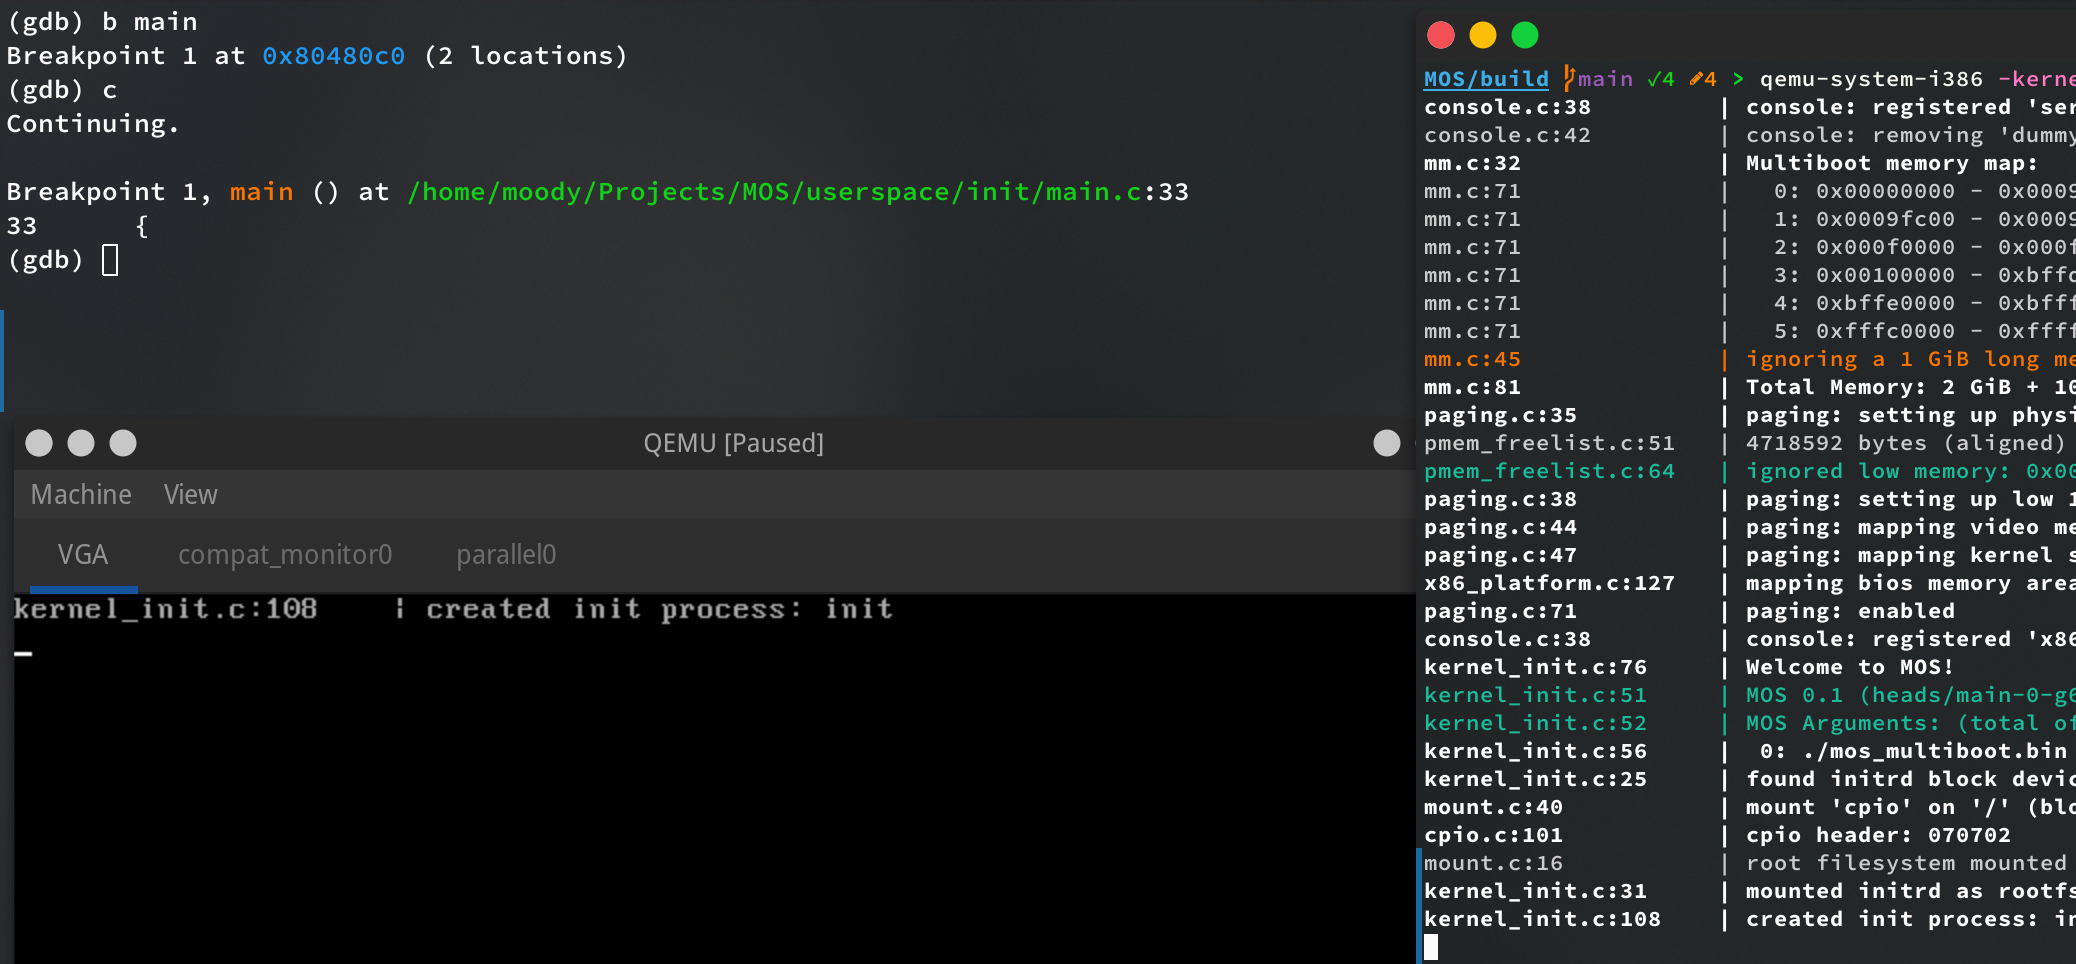
\includegraphics[width=\textwidth]{assets/c1.gdb-paused.png}
    \caption{GDB Paused at \texttt{main}}
    \label{fig:gdb-paused}
\end{figure}

\subsection{(Optional) Configure your IDE for Future Debugging} \label{sec:ide-config}

\begin{note}
    \item I personally use VSCode, thus only the VSCode part will be covered here. If you are
    using any other IDE (e.g. CLion), things \textbf{may} be different, but the underlying idea
    of remote debugging should be the same.

    \item IDEs are updating very fast, so the screenshots \textbf{may} be outdated. Ask me if you
    have any questions.
\end{note}

As you may (or may not) realize, attaching GDB to QEMU is basically same as remote debugging, so
we can configure our IDE to do this automatically. But notice that:

\begin{itemize}
    \item Use \texttt{i686-elf-gdb} instead of the default \texttt{gdb}
    \item We need to specify the \texttt{gdbinit} file.
\end{itemize}

\subsubsection{Prepared VSCode Setup} \label{sec:vscode-config}

\begin{tip}
    \item There are several suggested VSCode extensions:
    \begin{itemize}
        \item \texttt{C/C++} for C/C++ support
        \item \texttt{clangd} for C/C++ language server
        \item \texttt{CMake} for CMake support
    \end{itemize}
    \item \texttt{tmux} is also required for this setup.
\end{tip}

To use a prepared setup for VSCode, see the \texttt{launch.json} file in the \texttt{.vscode}
directory, which is also my personal configuration for debugging MOS.

Simply press \texttt{F5}, a QEMU window will pop up and you'll see the kernel booting up, with
the breakpoints you set in your IDE as shown in Figure \ref{fig:vscode-debugging}.

In this setup, you can also use \texttt{tmux attach-session -t mos\_kernel\_debug} to attach to the serial
port.

\begin{figure}[ht]
    \centering
    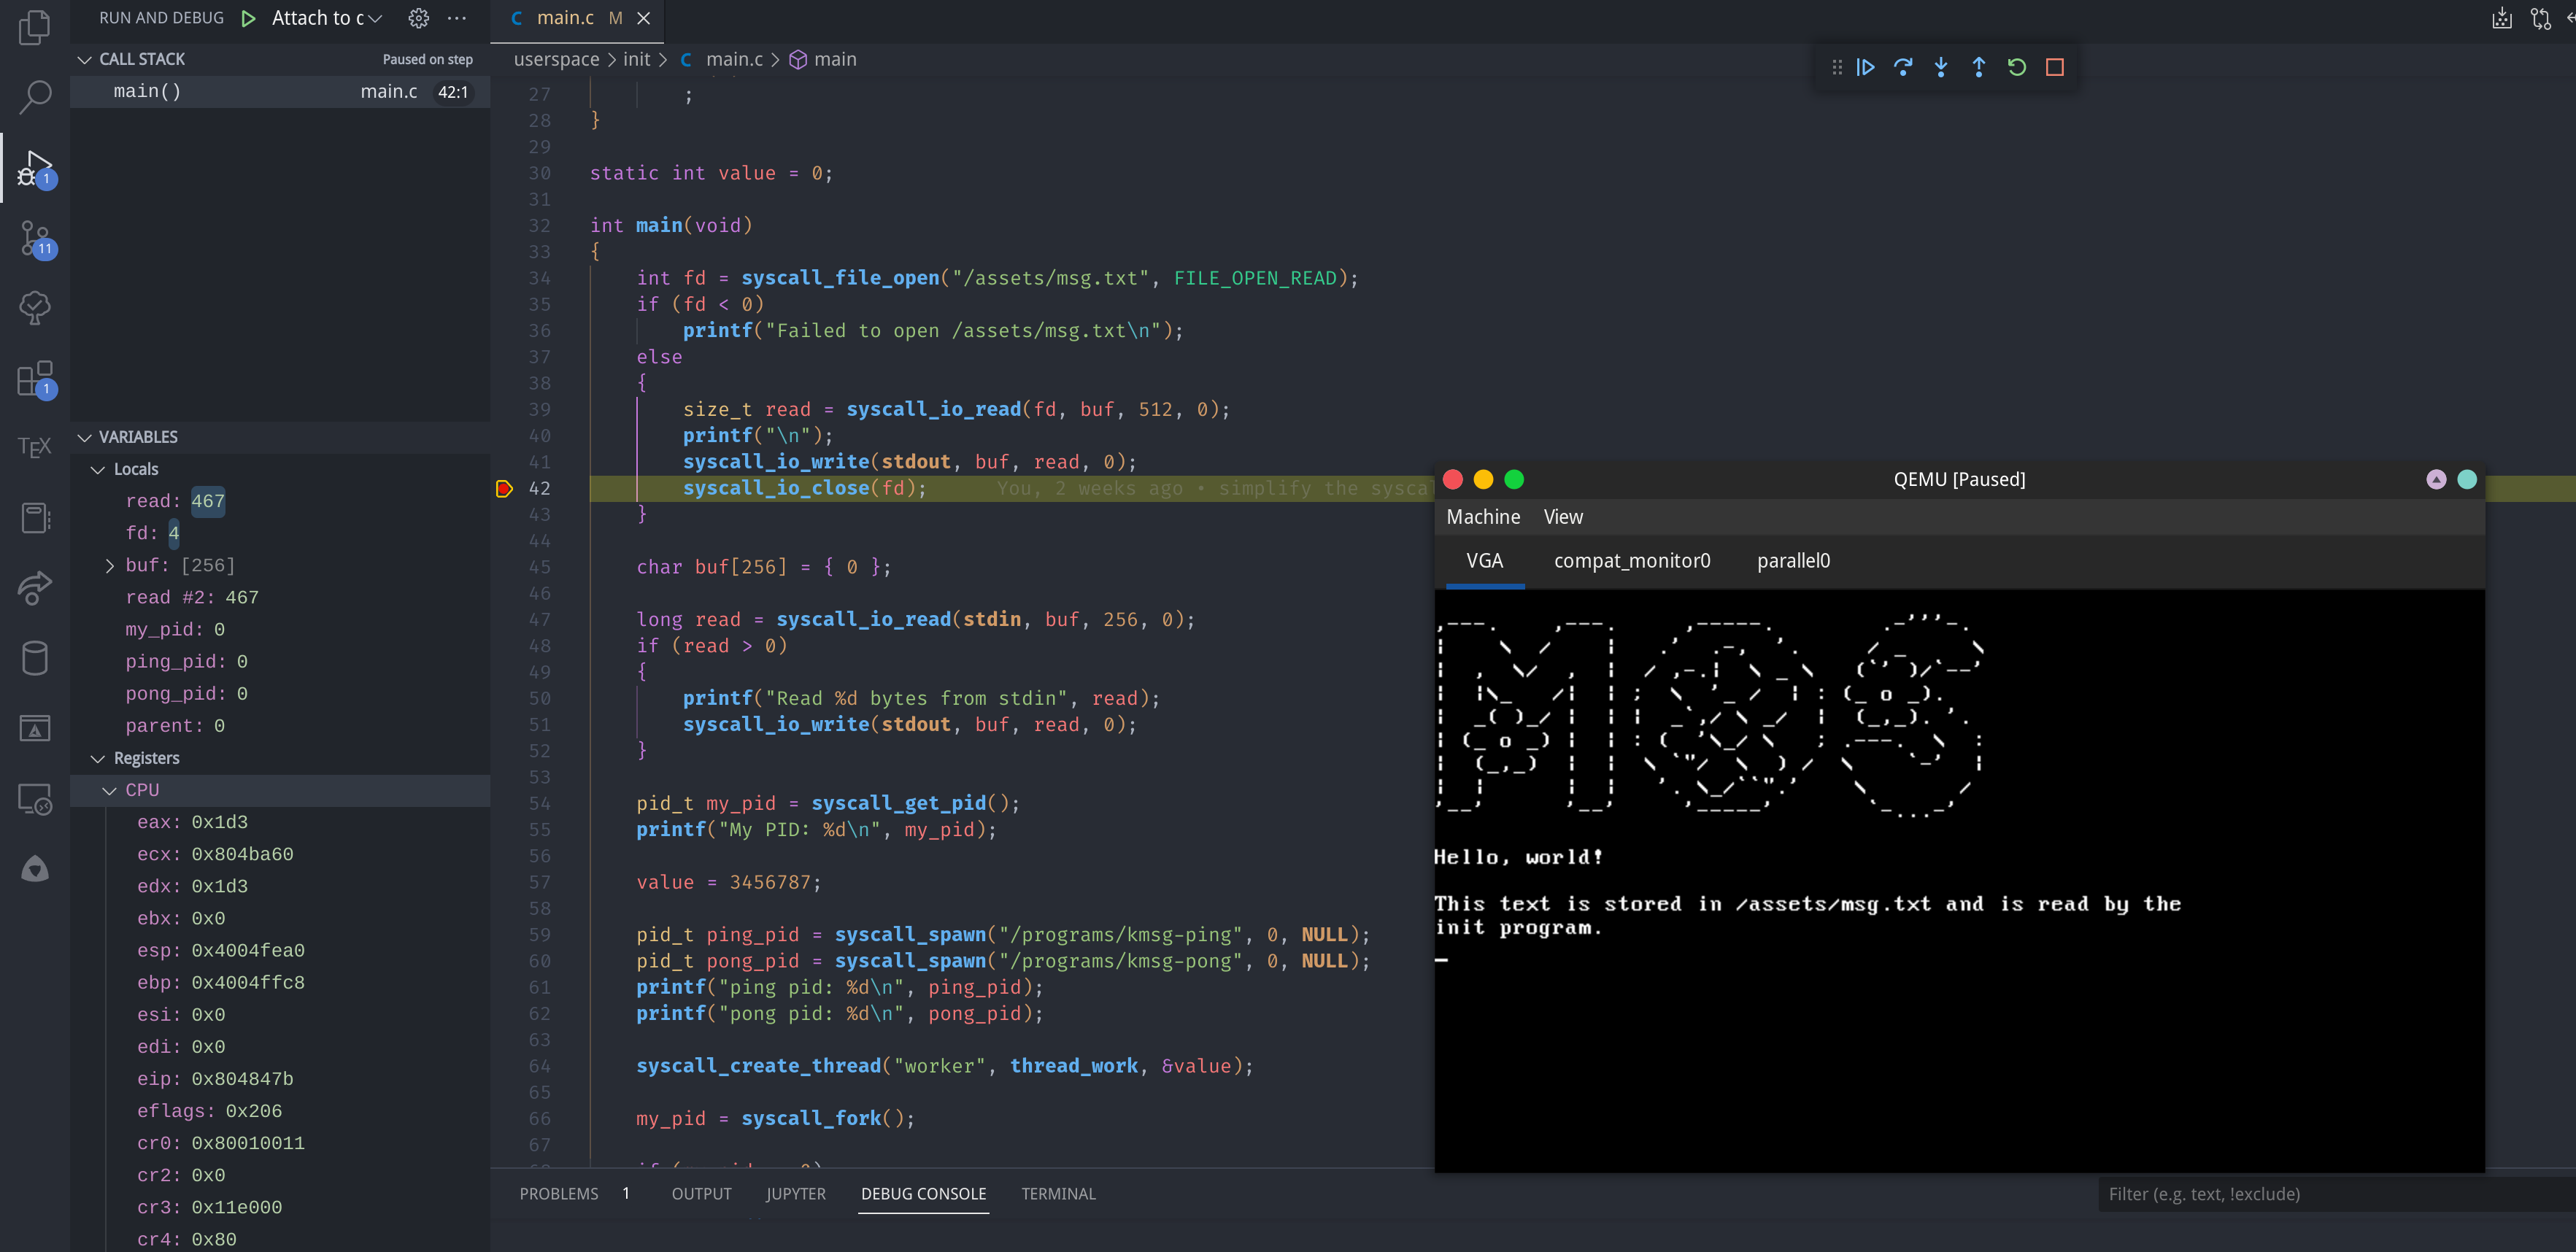
\includegraphics[width=\textwidth]{assets/c1.vscode-debugging.png}
    \caption{VSCode Debugging MOS}
    \label{fig:vscode-debugging}
\end{figure}

\subsection{Summary}

In this section, we've configured the cross-compiler, the build system and (possibly) the IDE for
our future MOS kernel development. We've also learned how to debug MOS kernel using QEMU and GDB.

Below are some exercises for you to practice and test your environment setup.

\begin{exercise}
    \item In the \texttt{mos\_start\_kernel} function (in \texttt{kernel/kernel\_init.c}), you'll find
    texts like `Welcome to MOS!'. Add some code here to print out your name with some other information.
    e.g. `This is [YOUR NAME]'s own version of MOS!'

    Compile and run the kernel, do you see your name printed out?

    \begin{tip}
        \item There are various ways to print out strings in MOS kernel, you can either of:
        \texttt{printk}, \texttt{pr\_info}, \texttt{pr\_info2}, \texttt{pr\_emph}, \texttt{pr\_warn},
        \texttt{pr\_emerg} or \texttt{pr\_fatal}, they have similar usage like \texttt{printf}.
        \item Can you spot the difference between \texttt{pr\_info} and \texttt{pr\_info2}?
    \end{tip}

    \item Try to set a breakpoint somewhere in the \texttt{mos\_start\_kernel} function, start debugging
    the kernel and see if it works.

    \item Optionally, try play with different CMake options, like \texttt{MOS\_DEBUG\_ALL}. See what happens to the
    kernel log.
\end{exercise}
